\documentclass[landscape]{article}
\usepackage[a4paper,margin=3mm,landscape]{geometry}
\usepackage[scaled=0.92]{helvet}
\usepackage{multicol, multirow}
\usepackage{makecell}
\usepackage{array} 
\usepackage[table]{xcolor}
\usepackage{enumitem} 
\usepackage{amssymb}
\usepackage{graphicx}
\usepackage{newlfont}
\usepackage{stix}
\setlength{\multicolsep}{6.0pt plus 2.0pt minus 1.5pt}
\setlist{nosep}

\graphicspath{{./images/}}

\pdfinfo{
    /Title (CS2102 Cheatsheet.pdf)
    /Creator (TeX)
    /Producer (pdfTeX 1.40.0)
    /Author (Selwyn Ang)
    /Subject (CS2102)
    /Keywords (CS2102, Cheatsheet, NUS, Database Systems) 
}

% Turn off header and footer
\pagestyle{empty}


\makeatletter
\DeclareRobustCommand\smaller{\@setfontsize\smaller{6pt}{6.5pt}}
\makeatother

% redefine section commands to use less space
\makeatletter
\renewcommand{\section}{\@startsection{section}{1}{0mm}%
  {-0.1ex plus -0.1ex minus -0.1ex}%
  {0.1ex plus .1ex minus 0.1ex}%
{\normalfont\small\bfseries}}
\renewcommand{\subsection}{\@startsection{subsection}{2}{0mm}%
  {-0.1ex plus -0.1ex minus -0.1ex}%
  {0.1ex plus .1ex minus 0.1ex}%
{\normalfont\scriptsize\bfseries}}
\renewcommand{\subsubsection}{\@startsection{subsubsection}{3}{0mm}%
  {-0.1ex plus -0.1ex minus -0.1ex}%
  {0.1ex plus .1ex minus 0.1ex}%
{\normalfont\smaller\bfseries}}%
\makeatother



\renewcommand{\familydefault}{\sfdefault}
\renewcommand\rmdefault{\sfdefault}
%  makes nested numbering (e.g. 1.1.1, 1.1.2, etc)
\renewcommand{\labelenumii}{\theenumii}
\renewcommand{\theenumii}{\theenumi.\arabic{enumii}.}
\renewcommand\labelitemii{•}
\renewcommand\labelitemiii{•}

\setlength{\parindent}{0pt}
\setlength{\parskip}{0pt plus 0.5ex}
\setlength{\columnsep}{0.2cm}
%% adjust spacing for all itemize/enumerate
\setlength{\leftmargini}{0.5cm}
\setlength{\leftmarginii}{0.5cm}
\setlist[itemize,1]{leftmargin=2mm,labelindent=1mm,labelsep=1mm}
\setlist[itemize,2]{leftmargin=2mm,labelindent=1mm,labelsep=1mm}
\setlist[itemize,3]{leftmargin=2mm,labelindent=1mm,labelsep=1mm}
\setlist[enumerate,1]{leftmargin=2mm,labelindent=1mm,labelsep=1mm}
\setlist[enumerate,2]{leftmargin=2mm,labelindent=1mm,labelsep=1mm}
\setlist[enumerate,3]{leftmargin=2mm,labelindent=1mm,labelsep=1mm}

% tightcenter
\newenvironment{tightcenter}{%
  \setlength\topsep{0pt}
  \setlength\parskip{0pt}
  \begin{center}
    }{%
  \end{center}
}

% boxed
\newenvironment{tightbox}{%
  \setlength\topsep{0pt}
  \setlength\parskip{0pt}
  \begin{center}
    \begin{tabular}{|@{\hspace{\dimexpr\fboxsep+0.5\arrayrulewidth}}c@{\hspace{\dimexpr\fboxsep+0.5\arrayrulewidth}}|}
      \hline
    }
    {%
    \\ \hline
    \end{tabular}
  \end{center}
}

% fixed width box
\newenvironment{fixedbox}[1][0.7]{
  \setlength\topsep{0pt}
  \setlength\parskip{0pt}
  \begin{center}
    \begin{tabular}{|>{\centering\arraybackslash}m{#1\linewidth}|}
    \hline
  }{
  \\ \hline
  \end{tabular}
  \end{center}
}

% definition of a new term
\usepackage{soul}
\definecolor{paleyellow}{RGB}{251,243,218}
\newcommand{\definition}[2][]{\sethlcolor{paleyellow}\hl{\textbf{#2}} #1  $\rightarrow$}
% inline definition
\newcommand{\ildefinition}[1]{\sethlcolor{paleyellow}\hl{\textbf{#1}}}

% important note (attention)
\newcommand{\attention}{{\color{red}\textbf{! }}}

% nice proof
\newenvironment{niceproof}[1][Proof]
{%
  \sbox0{\textit{#1}. }%
  \list{}{\labelwidth\wd0 \leftmargin\wd0 \labelsep 0pt }
\item[\usebox0]}
  {\endlist}


\usepackage{color, soul}
\usepackage{listings}
\usepackage{inconsolata}

\definecolor{codegreen}{rgb}{0,0.6,0}
\definecolor{codegray}{rgb}{0.5,0.5,0.5}
\definecolor{codepurple}{HTML}{C42043}
\definecolor{backcolour}{HTML}{F2F2F2}
\definecolor{bookColor}{cmyk}{0,0,0,0.90}

\newcommand{\code}[1]{\texttt{\sethlcolor{backcolour}\hl{$\,$#1$\,$}}}

% SQL code blocks
% define SQL styles
\lstdefinestyle{mySQL}{%
  language=SQL,
  backgroundcolor=\color{backcolour},
  commentstyle=\color{codegreen},
  keywordstyle=\color{codepurple},
  numberstyle=\numberstyle,
  stringstyle=\color{codepurple},
  basicstyle=\scriptsize\ttfamily,
  breaklines=true,
}



% --------------------------------------------------------

\begin{document}
\raggedright
\smaller
\begin{multicols*}{5}
    \setlength{\columnseprule}{0.25pt}

    \begin{tightcenter}
        \fbox{%
          \parbox{0.8\linewidth}{\centering \textcolor{black}{
              {\Large\textbf{CS2102 Finals}}
            \\ \normalsize{AY23/24 SEM 2}}
            \\ {\footnotesize \textcolor{gray}{github/SelwynAng}}
          }%
        }
    \end{tightcenter}
    
    \section{Relational Model}
    \subsection{DBMS}
    \begin{itemize}
      \item \textbf{Transactions:} Finite sequence of operations \& constitutes smallest logical unit of work from application perspective
      \item \textbf{Properties of Transactions:}
      \begin{enumerate}
        \item \underline{Atomicity:} Either all effects of Transaction are reflected in database or none
        \item \underline{Consistency:} Transaction guarantees to yield correct state of database
        \item \underline{Isolation:} Transaction is isolated from effects of concurrent Transactions
        \item \underline{Durability:} After commit of Transaction, effects are permanent
      \end{enumerate}
      \item \textbf{Equivalent Transaction}: 2 executions are equivalent if they have same effect on database
      \item \textbf{Serialisability:} Concurrent execution of a set of transactions is serialisable if execution is equivalent to some serial execution of the same set of Transactions
    \end{itemize}

    \subsection{Relational Model}
    \begin{multicols}{2}
      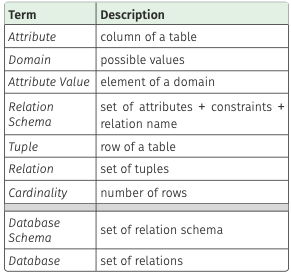
\includegraphics[width=1.0\linewidth]{1_relational_model.png}
      \columnbreak
        \\ \underline{Relational Schema:} Defines a relation, specifies attributes (columns), data constraints, name 
        \begin{itemize}
          \item $R(A_1, A_2, \dots A_3)$: relation schema with name $R$ and $n$ attributes $A_1, A_2, \dots, A_n$
          \item Eg. \verb|Employees(id:INT,| \verb|name:TEXT, dob:TEXT)|
        \end{itemize}
    \end{multicols}
    \underline{Domain:} Set of atomic values, including NULL
    \begin{itemize}
      \item $dom(A_i)$ = set of possible values for $A_i$
      \item $\forall$ value $v$ of attribute $A_i$, $v \in \{dom(A_i \cup \{null\})\}$
    \end{itemize}

    \subsection{Keys}
    \begin{itemize}
      \item \textbf{Superkey:} Subset of attributes that UNIQUELY IDENTIFIES  a tuple in a relation
      \item \textbf{Key:} Superkey that is also MINIMAL (No proper subset of key is a superkey)
      \item \underline{Properties of Superkeys \& Keys:}
      \begin{enumerate}
        \item If (A,B,C) is DEFINITELY superkey $\rightarrow$ (A,B,C,D) is superkey
        \item If (A,B,C) is DEFINITELY key $\rightarrow$ (A,B,C) is superkey
        \item If (A,B) is DEFINITELY superkey $\rightarrow$ (A,B,C) is NOT a key
        \item If (A,B) is DEFINITELY key $\rightarrow$ possible (B,C,D) is also key
        \item Every relation has $\geq$ 1 superkey
      \end{enumerate}
      \item \textbf{Candidate Key:} Set of all keys of a given relation
      \item \textbf{Primary Key:} A selected candidate key (attributes CANNOT be NULL, is underlined in schema notation)
      \item \textbf{Foreign Key:} Subset of attributes of relation $R_1$ that refers to Primary Key of relation $R_2$
      \begin{itemize}
        \item $R_1$ is referencing relation, $R_2$ is referenced relation
        \item $R.sid \rightarrow S.id$: $R.sid$ is a FK referencing PK $id$ in $S$
        \item FK in $R_1$ must appear as PK in $R_2$ OR be NULL/tuple containing at least 1 NULL value
        \item A referencing relation can be a referenced relation for different foreign key $\vert$ Referencing relation \& referenced relation can be same relation
      \end{itemize}
    \end{itemize}

    \section{SQL}
    \subsection{Three-valued Logic / Handing NULLs}
    \begin{itemize}
      \item \textbf{Logical Operations}
      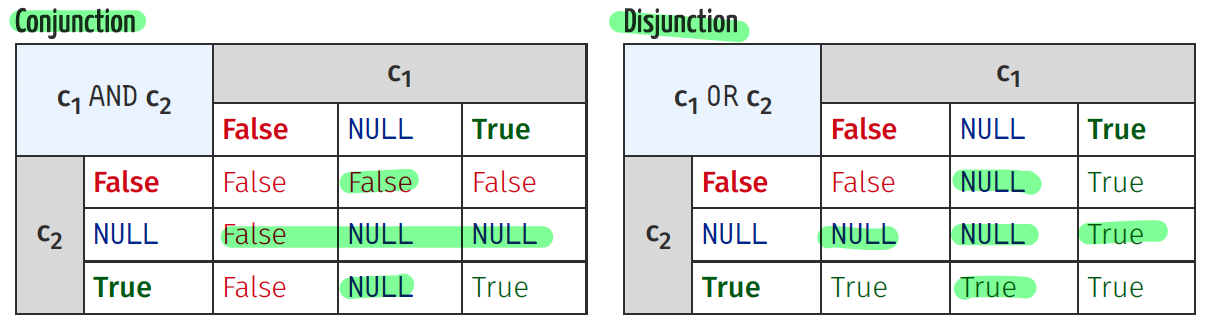
\includegraphics[width=1.0\linewidth]{2_three_valued_logic.png}
      \begin{itemize}
        \item \textbf{Implication:} $C_1 \rightarrow C_2$ == $(\sim C_1) \vee C_2$
        \item $\sim NULL$ == $NULL$
      \end{itemize}
      \item \textbf{Relational Operations:} Any relational operations with $NULL$ produced $NULL$ values (Eg. $\leq$, $=$, $!=$)
      \item \textbf{Arithmetic Operations:} Any arithmetic operations with $NULL$ produces $NULL$ values
      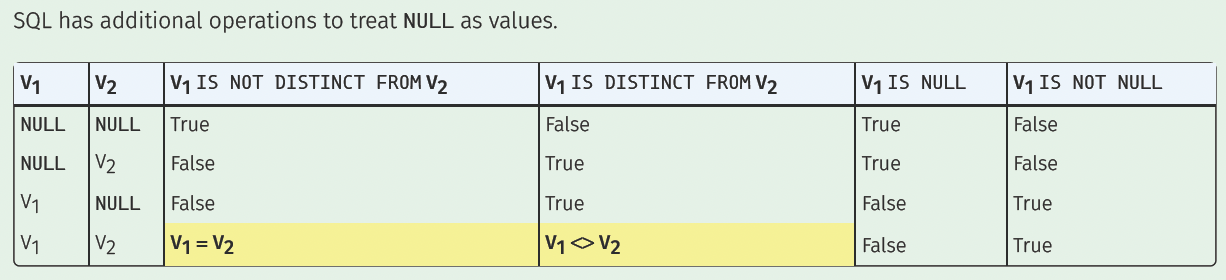
\includegraphics[width=1.0\linewidth]{3_nulls.png}
      \item \textbf{IS NULL vs = NULL (in WHERE clause):} IS NULL will select NULL values $\vert$ = NULL will not select any NULL values (NULL = NULL $\rightarrow$ NULL, nothing will be selected by Principle of Acceptance)
      \item \textbf{DISTINCT keyword (in SELECT clause):} DISTINCT checks for distinct rows using IS DISTINCT FROM (Duplicate NULL values are removed)
      \item \textbf{Empty \& NULL Semantics in Aggregate functions}
      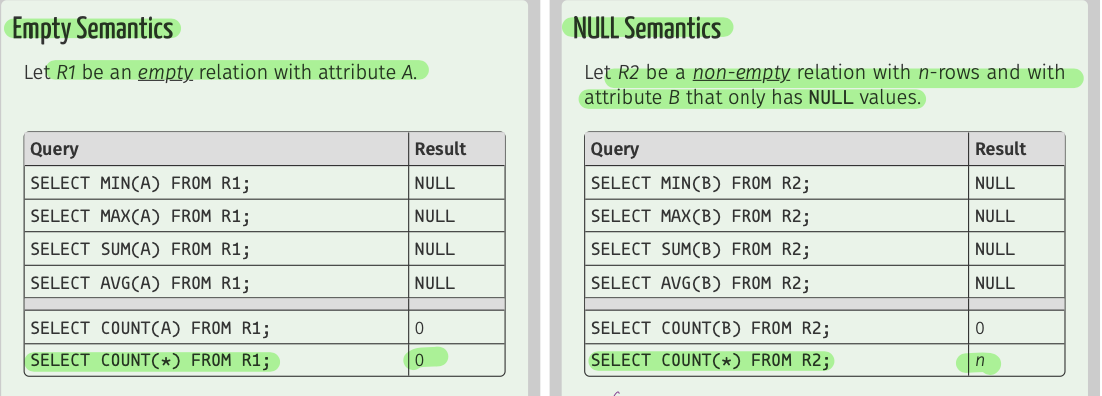
\includegraphics[width=1.0\linewidth]{4_empty_null_semantics.png}

      \subsection{Integrity Constraints}
      \begin{itemize}
        \item \textbf{Principle of Rejection:} Integrity Constraints follow POR (Rejects insertion if condition evaluates to FALSE, Insertion is still done if condition is NULL) 
      \end{itemize}
      \begin{enumerate}
        \item \underline{NOT NULL:} Rejects insertion if value at specified column is NULL (Condition: IS NOT NULL)
        \item \underline{UNIQUE:} Rejects insertion if there are other rows where values are equal (Condition: $x.A_i <> y.A_i$) $\vert$ Can have multiple NULL values since NULL $<>$ NULL == NULL
        \item \underline{Primary Key:} Equivalent to UNIQUE \& NOT NULL $\vert$ If one of the attributes is NULL, entire tuple is rejected
        \item \underline{Foreign Key:} Rejects insertion if tuple does not exist in referenced relation AND is NOT NULL
        \begin{itemize}
          \item NO ACTION: Rejects delete/update if it violates constraints
          \item CASCADE: Propagates delete/update to referencing tuples
          \item SET DEFAULT: Updates FK of referencing tuples to default value
          \item SET NULL: Updates FK of referencing tuples to NULL value
        \end{itemize}
        \item \underline{CHECK:} Rejects insertion if condition is FALSE
      \end{enumerate}
    \end{itemize}

    \subsection{Deferrable Constraints}
    \begin{itemize}
      \item \textbf{Default Behaviour:} Constraints are checked immediately at end of SQL statement $\rightarrow$ Violation of 1 of the statements will cause whole transaction to roll black
      \item \textbf{Benefit:} Allow cyclic FK constraints
    \end{itemize}
    \begin{enumerate}
      \item \underline{NOT DEFERRABLE:} Constraint checks are not deferred at all
      \item \underline{DEFERRABLE INITIALLY DEFERRED:} Constraint checks are deferred right at the start
      \item \underline{DEFERRABLE INITIALLY IMMEDIATE:} Constraint checks are not deferred until DEFERRED keyword in transaction (Defer constraints on demand)
    \end{enumerate}

    \subsection{Set Operations}
    \begin{itemize}
      \item \textbf{Union Compatible:} 2 relations are union-compatible if (1): Both have same \# of attributes, (2): Corresponding attributes have same or compatible domains (Similar to function signatures where number, order \& type matters)
      \item \textbf{Remove Duplicates:} \verb |UNION, INTERSECT, EXCEPT|
      \item \textbf{Keep Duplicates:} \verb|UNION ALL, INTERSECT ALL, EXCEPT ALL| (Treats each element as distinct element)
    \end{itemize}
    
    \subsection{Subqueries}
    \begin{itemize}
      \item Appears in \verb|SELECT, FROM, WHERE|
      \item \textbf{IN/NOT IN}: Subquery must return exactly 1 column $\vert$ If expression matches any subquery row $\rightarrow$ IN returns TRUE, NOT IN returns FALSE $\vert$ If subquery evaluates to empty table $\rightarrow$ IN returns FALSE, NOT IN returns TRUE
      \item \textbf{EXISTS/NOT EXISTS}: Subquery may return any \# of columns $\vert$ If expression matches any subquery row $\rightarrow$ EXISTS returns TRUE, NOT EXISTS returns FALSE $\vert$ If subquery evaluates to empty table, EXISTS returns FALSE, NOT EXISTS returns TRUE $\vert$ Only emptiness of subquery matters (Use \verb|SELECT 1|)
      \item \textbf{ANY/ALL}: Subquery must return exactly 1 column $\vert$ ANY returns TRUE if comparison is true to $\geq$ 1 row, ALL returns TRUE if comparison is true to all rows  $\vert$ If subquery evaluates to empty table, ANY returns FALSE, ALL returns TRUE
    \end{itemize}

    \subsection{Conceptual Evaluation}
    \begin{enumerate}
      \item \textbf{FROM}: Compute cross product/JOINs of all Tables in FROM clause
      \item \textbf{WHERE}: Keep tuples that evaluates to TRUE on the WHERE condition (WHERE follows Principle of Acceptance $\vert$ Cannot use aggregate directly in WHERE, but can have sub-query which contains aggregate in WHERE)
      \item \textbf{GROUP BY}: Partition table into groups w.r.t grouping attributes (Application of aggregate functions are over each group $\rightarrow$ 1 result tuple per group)
      \item \textbf{HAVING}: Keep groups that evaluates to TRUE on the HAVING condition (Conditions typically involve aggregates)
      \item \textbf{SELECT}: Remove all attributes not specified in SELECT clause (Remove duplicates if DISTINCT)
      \item \textbf{ORDER BY}: Sort tables based on specified attributes
      \item \textbf{LIMIT/OFFSET}: Keep tuples based on their order in table
    \end{enumerate}
    \textbf{Restriction to SELECT/HAVING clauses upon GROUP BY}: If column $A_i$ of table R appears in SELECT/HAVING clause, $A_i$ must appear in GROUP BY clause OR $A_i$ appear as input of aggregate function in SELECT/HAVING clause OR PK of R appears in GROUP BY clause

    \subsection{Special Functions}
    \begin{enumerate}
      \item \textbf{Patter Matching:} \_ matches any single character, \% matches any sequence of 0 or more characters (eg. \verb|WHERE pizza LIKE 'Ma%a'|)
      \item \textbf{COALESCE}: Returns 1st non-NULL value in list of input arguments, returns NULL if all values in list are NULL
      \item \textbf{NULLIF:} Returns NULL if $value_1$ = $value_2$, otherwise return $value_1$
    \end{enumerate}

    \subsection{Universality}
    \begin{itemize}
      \begin{multicols}{2}
        \item \textbf{Double Negation Method:} $\forall x: Exist(x)$ == $\sim\exists x: \sim Exist(x)$
        \item Eg. Restaurants that sells ALL pizzas liked by 'Homer' == There does not exist pizza that 'Homer' likes \& not sold by the restaurant
        \columnbreak
        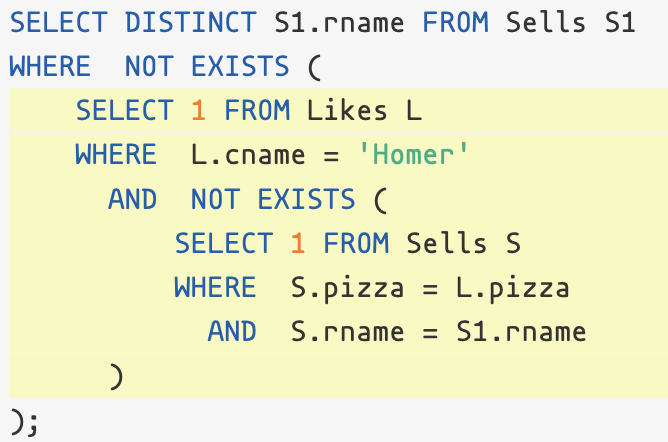
\includegraphics[width=1.0\linewidth]{5_double_negation.png}
      \end{multicols}
      \item \textbf{Cardinality Method:} \\ $S \subseteq R$ $\rightarrow$ $\mid R \cup S \mid = \mid R \mid$, $\mid R \cap S \mid = \mid S \mid$ \\ $R \equiv S$ $\rightarrow$ $\mid R \cup S \mid = \mid R \cap S \mid$
    \end{itemize}

    \subsection{Recursive CTE}
    \underline{Eg.} Find all MRT stations that can be reached from NS1 in at most 3 stops \\
      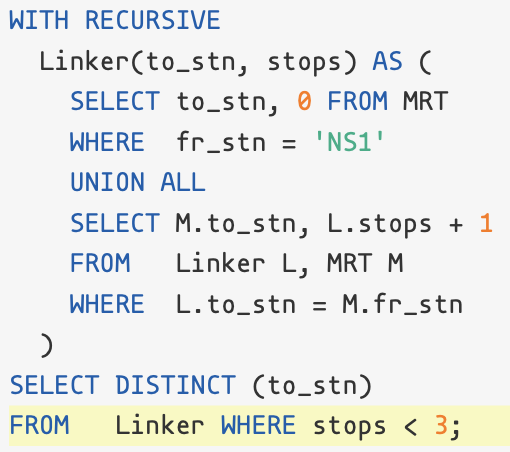
\includegraphics[width=0.45\linewidth]{6_recursive_cte_eg.png}

    \section{Entity Relationship Model}
    \subsection{Entity Relationship}
    \begin{itemize}
      \item \textbf{Entities:} Nouns (Rectangles), \textbf{Relationships:} Verbs (Diamonds)
      \item \textbf{Attributes:} Describe info about entities \& relationships
      \begin{enumerate}
        \item \underline{Key attribute:} Uniquely identifies each Entity
        \item \underline{Composite attribute:} Composed of multiple other attributes
        \item \underline{Multi-valued attributes:} 1 or more values for a given Entity
        \item \underline{Derived attributes:} Derived from other attributes
        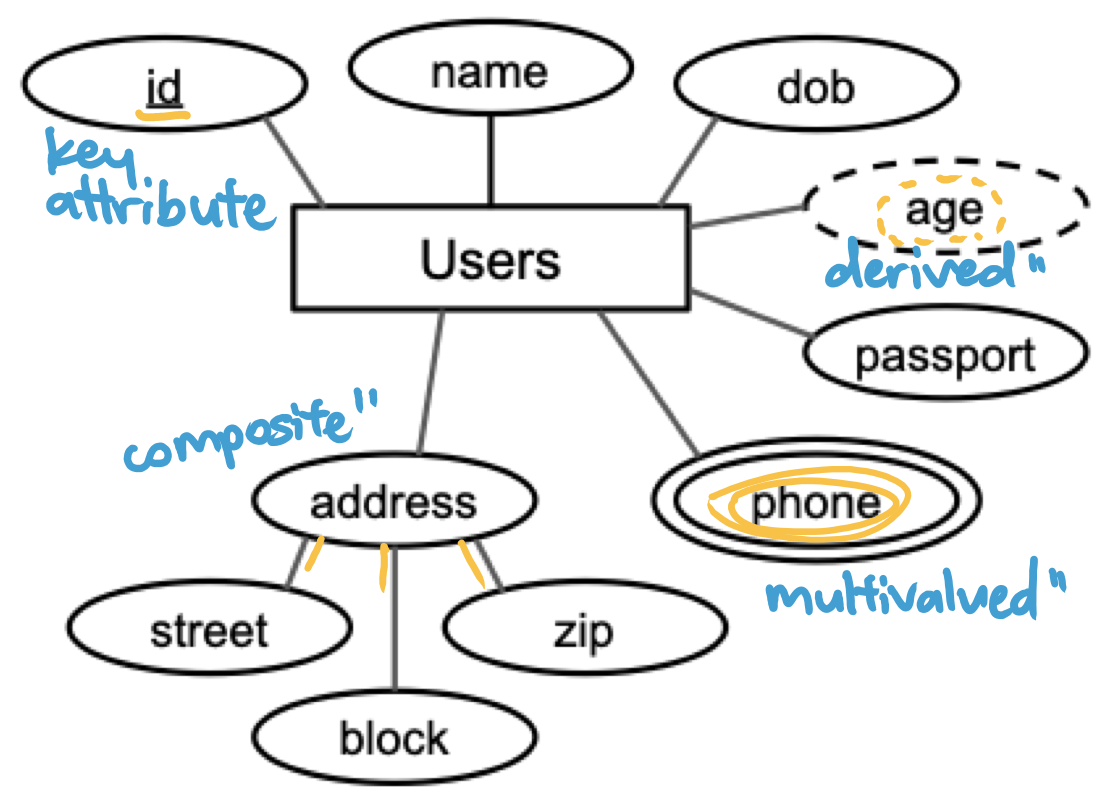
\includegraphics[width=0.55\linewidth]{7_attribute_subtypes.png}
      \end{enumerate}
      \item \textbf{Degrees of Relationship Sets:} \# of entity sets (can be non-unique) involved in relationship set
    \end{itemize}

    \subsection{Relationship Constraints}
    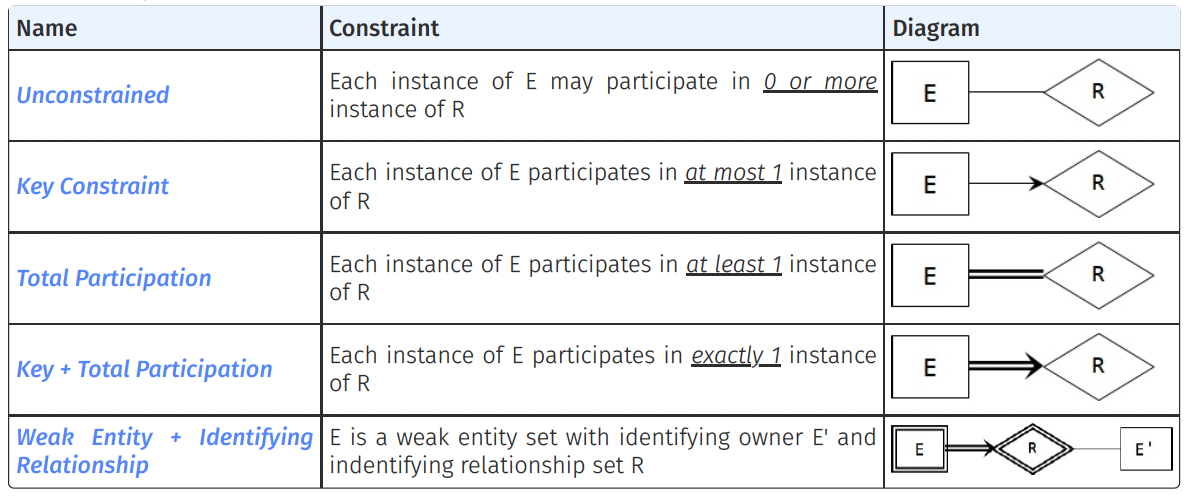
\includegraphics[width=1.0\linewidth]{8_summary_relationship_constraints.png}
    \textbf{Weak Entity Set:} An entity set that does not have its own key (Has partial key that cannot uniquely identify an entity) $\rightarrow$ Needs help of key from \underline{Owning Entity Set} to uniquely identify an entity
    
    \subsection{Relational Mapping (ER to Schema)}
    \textbf{Entity Set}
    \begin{enumerate}
      \item \underline{Name} of entity set $\rightarrow$ Name of table
      \item \underline{Attribute} of entity set $\rightarrow$ Column of table
      \item \underline{Key attribute} of entity set $\rightarrow$ PK of table
      \item \underline{Derived attribute} of entity set $\rightarrow$ Should not appear in table
      \item \underline{Composite attribute} of entity set $\rightarrow$ Converted into decomposed attributes in table
      \item \underline{Multi-valued attribute} of entity set $\rightarrow$ Converted into seq. of single-valued attributes OR Create another table with FK constraint
    \end{enumerate}
    \textbf{Relationship Set}
    \begin{enumerate}
      \item \underline{Many-to-Many Relationship:} Relationship Set Schema should have its PK including PKs of both entities
      \item \underline{Many-to-One Relationship:} 
      \begin{itemize}
        \item \textit{Separate Tables strategy:} Relationship Set Schema should have PK of One-Set as its PK to enforce upper bound of 1 \&  PK of Many-Set in Relationship Set should be NOT NULL to prevent redundant info
        \item \textit{Combined Tables strategy:} Combine Relationship Set with One-Set, PK of merged set is PK of One-Set, PK of Many-Set in merged set can be NULL
      \end{itemize}
      \item \underline{One-to-One Relationship:}
      \begin{itemize}
        \item \textit{No Relationship Set strategy:} PK of each entity set is a UNIQUE FK in other set
        \item \textit{3 Table strategy:} Relationship Set Schema has its PK as PK of 1 of the entity set, other entity set's PK appears in Relationship Set Schema as a UNIQUE, NOT NULL FK (candidate key)
      \end{itemize}
      \item \underline{Key + Total Relationship:} Combine Relationship Set with KeyTotal-Set, PK of merged set is PK of KeyTotal-Set, PK of Many-Set in Relationship Set must be NOT NULL
      \item \underline{Weak Entity Set Relationship:} Combine Relationship Set with Weak Entity Set, PK of merged set is combination of Owning Entity Set's PK \& Weak Entity Set's PK, PK of Owning Entity Set appears as FK in merged set with ON DELETE/UPDATE CASCADE 
    \end{enumerate}
    \textbf{NOTE:} Total Participation Constraint in ER model cannot be enforced by schema

    \subsection{ISA Hierarchy}
    \begin{itemize}
      \item Subclass must be uniquely identified by same key attributes of superclass (subclass keys should not be shown in ER diagram)
      \item Subclass may have additional attribute \& involved in additional relationship
      \item \textbf{Schema Syntax:} Subclass has Superclass's PK as its PK \& FK (along with ON DELETE CASCADE)
      \begin{multicols}{2}
        \noindent
        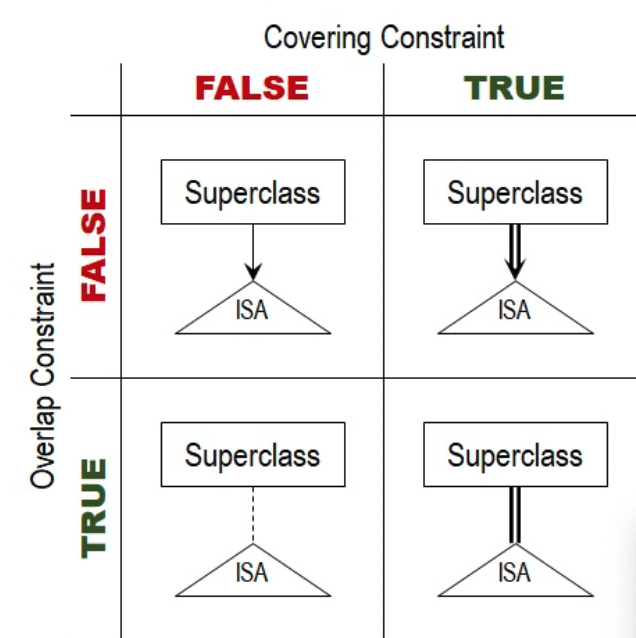
\includegraphics[width=0.9\linewidth]{9_ISA.png}
        \columnbreak
        \begin{enumerate}
          \item Overlap Constraint (Upper bound): Can a superclass belong to multiple subclasses? FALSE sets Upper bound = 1 (Key constraint)
          \item Covering Constraint (Lower bound): Must a superclass belong to $\geq$ 1 subclass? TRUE sets Lower bound = 1 (Total Participation constraint)
        \end{enumerate}
      \end{multicols}
    \end{itemize}

    \subsection{Aggregation}
    \begin{itemize}
      \item Aggregate is a relationship set \& entity set
      \item Key attributes are formed from relationship set
    \end{itemize}
    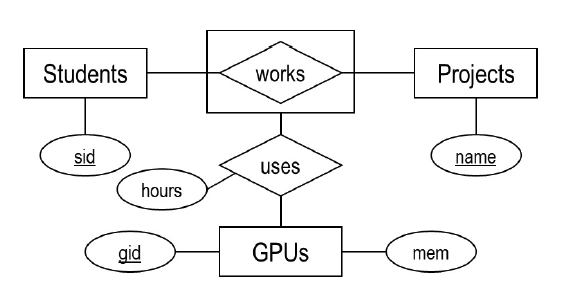
\includegraphics[width=0.55\linewidth]{10_aggregate_diagram.png}
    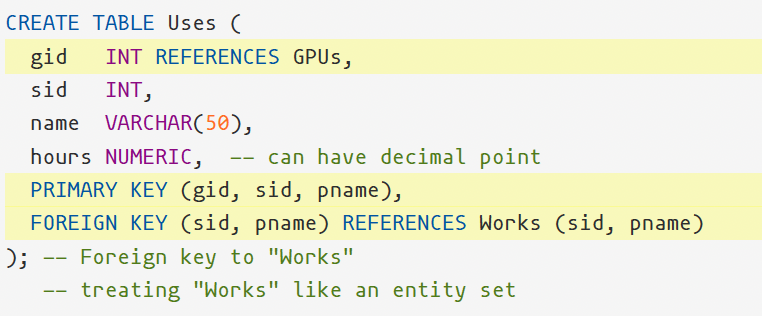
\includegraphics[width=0.75\linewidth]{11_aggregate_schema.png}
    \begin{multicols}{2}
      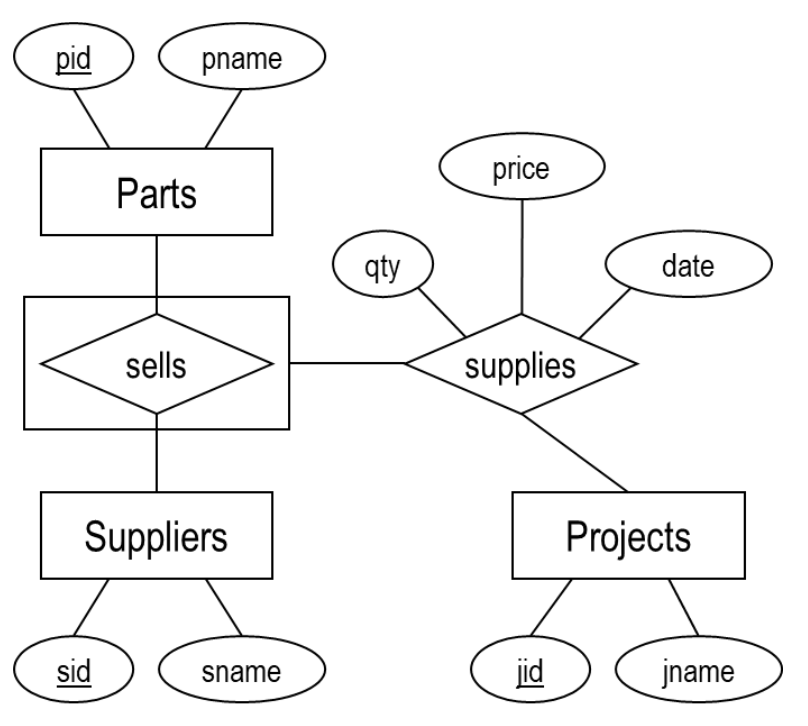
\includegraphics[width=0.8\linewidth]{12_aggregate_example.png}
      \begin{itemize}
        \item Supplier can sell Part without being used by a Project
        \item Aggregate's relationship set depicts necessary relationship btw. 2 entity sets
        \item Aggregate's entity set depicts optional relationship
      \end{itemize}
    \end{multicols}

    \section{Relational Algebra}
    \subsection{Algebra}
    \textbf{Closure:} A set of values is closed under the set of operators if any combination of the operators produces only values in the given set (Relations are closed under Relational Algebra)
    
    \subsection{Unary Operators}
    \textbf{Selection Operator ($\sigma$)}
    \begin{itemize}
      \item $\sigma_{[c]}(R)$ : Selects all tuples from relation $R$ (ROWS) that satisfies the selection condition $c$ based on Principle of Acceptance
      \item $c$ is a condition that returns a boolean (potentially NULL), $c$ must specify only attributes in $R$
      \item \underline{Precedence:} $(), op, \neg , \wedge , \vee$
      \item Can be mapped to \verb|WHERE| clause of SQL
      \item \underline{Properties:} Result have same schema as input relation $\vert$ \# of rows are often smaller
    \end{itemize}
    \textbf{Projection Operator ($\pi$)}
    \begin{itemize}
      \item $\pi_{[l]}(R)$ : Keeps only columns specified in ordered list $l$ and in same order 
      \item $l$ must specify only attributes in $R$, No operations \& duplicates in projection operator (eg. $\pi_{[A_1 + A_2]}(R)$, $\pi_{[A_1, A_1]}(R)$)
      \item $\pi_{[A_1, A_2]}(R) \neq \pi_{[A_2, A_1]}(R)$ (Order matters!!)
      \item Can be mapped to \verb|SELECT| clause in SQL
      \item \underline{Properties:} Resulting schema is as specified by $l$ without relation name $\vert$ \# of rows may be smaller (Relation is defined as set of tuples $\rightarrow$ Duplicate rows will be removed)
    \end{itemize}
    \textbf{Renaming Operator ($\rho$)}
    \begin{itemize}
      \item $\rho_{[r]}(R)$ : Renames all attributes mentioned in $r$ s.t. for each renaming $B_i \leftarrow A_i$, $A_i$ is renamed to $B_i$
      \item Can be mapped to \verb|AS| keyword in \verb|SELECT| in SQL
      \item \underline{Properties:} Resulting schema is old schema renamed by $r$ $\vert$ Order of column is unchanged (except for renaming) $\vert$ \# of rows remains the same
    \end{itemize}

    \subsection{Binary Operators}
    \textbf{SET Operators}
    \begin{itemize}
      \item $R \cap S$, $R \cup S$, $R - S$ (Relations must be union-compatible)
    \end{itemize}
    \textbf{PRODUCT Operators}
    \begin{itemize}
      \item $R \times S$ : Cross product of 2 relations is a relation formed by combining all pairs of tuples from 2 input relations
      \item Can be mapped to \verb|FROM| keyword in SQL
      \item \underline{Optimisation:} Cross product can be optimised by \verb|JOIN| operators, which combines cross product, selection \& projection (Avoids generating all $\vert R \times S \vert$ intermediate tuples)
    \end{itemize}
    \textbf{INNER JOIN Operators}
    \begin{enumerate}
      \item \textbf{$\theta$ Join:} $R \Join_{[\theta]}S$ = $\sigma_{[\theta]}(R \times S)$ (Cross product followed by selection)
      \item \textbf{Equi Join}: $R \Join_{[=]}S$ = Special $\theta$ Join where the only relational operator used is equality (All equi join is a $\theta$ join but not all $\theta$ join are equi join)
      \item \textbf{Natural Join:} $R \Join S$ = $\pi_{[l]} (\sigma_{[\theta]}(R \times S))$
      \begin{itemize}
        \item $l$ = $(Attr(R) \cap Attr(S)) + (Attr(R) - Attr(S)) + (Attr(S) - Attr(R))$ (Order matters, where common attributes are listed, then R's attributes, followed by S's attributes)
        \item $\theta$ = $\forall \in (Attr(R) \cap Attr(S)): R.A_i = S.A_i$ (All common attributes are equal)
      \end{itemize}
    \end{enumerate}
    \textbf{OUTER JOIN Operators}
    \begin{enumerate}
      \item \textbf{Semi Join:} $R \ltimes_{[\theta]}S$ = $\pi_{[Attr(R)]}(R \Join_{[\theta]}S)$ (Used to find non-dangling tuple)
      \\ NOTE: Semi Join projects R's attributes only, while normal Joins will project R and S's attributes
      \item \textbf{Dangles:} $dangle(R \Join_{[\theta]}S)$ = $R - R \ltimes_{[\theta]}S$
      \item \textbf{Left Outer Join:} $R_1 \leftouterjoin_{[c]}R_2$ = Inner Join $\cup$ Left Dangling Tuple = $R_1 \Join_{[c]} R_2 \cup (dangle(R_1 \Join_{[\theta]}R_2) \times (null(R_2))$
      \item \textbf{Right Outer Join:} $R_1 \rightouterjoin_{[c]}R_2$ = Inner Join $\cup$ Right Dangling Tuple = $R_1 \Join_{[c]} R_2 \cup ((null(R_1) \times dangle(R_2 \Join_{[\theta]}R_1))$
      \item \textbf{Full Outer Join:} $R_1 \fullouterjoin_{[c]}R_2$ = Inner Join $\cup$ Left Dangling Tuple $\cup$ Right Dangling Tuple = $R_1 \Join_{[c]} R_2 \cup (dangle(R_1 \Join_{[\theta]}R_2) \times (null(R_2)) \cup ((null(R_1) \times dangle(R_2 \Join_{[\theta]}R_1))$
    \end{enumerate}

    \subsection{Complex Expressions}
    \textbf{Equivalence VS Isomorphic}
    \begin{itemize}
      \item \underline{Equivalence ($\equiv$):} 2 relational algebra expressions are equivalent if both produces same result with same column order, possibly different row order
      \item \underline{Isomorphic ($\cong$):} 2 relational algebra expressions are isomorphic if both produces same result with possibly different column order, possibly different row order
    \end{itemize}
    \textbf{Special Properties}
    \begin{enumerate}
      \item $\sigma_{[\theta_1]}(\sigma_{[\theta_2]}(R)) \equiv \sigma_{[\theta_2]}(\sigma_{[\theta_1]}(R)) \equiv \sigma_{[\theta_1 \wedge \theta_2]}(R)$
      \item $\pi_{[l_1]}(\pi_{[l_2]}(R)) \nequiv \pi_{l_1}(R)$ unless $l_1 \subseteq l_2$
      \item $R \times S \cong S \times R$, $R \Join S \cong S \Join R$, $R \Join (S \Join T) \cong (R \Join S) \Join T$ (Different column order)
      \item $R \times (S \times T) \equiv (R \times S) \times T$ (Associative)
      \item $\pi_{[l]}(\sigma_{[\theta]}(R)) \nequiv \sigma_{[\theta]}(\pi_{[l]}(R))$ (Unless $\theta$ uses only attributes in $l$)
      \item $\sigma_{[\theta]}(R \times S) \nequiv \sigma_{[\theta]}(R) \times S$ (Unless $\theta$ uses only Attr($R$))
    \end{enumerate}

    \section{Functions \& Procedures}
    \subsection{Functions}
    \begin{itemize}
      \item Returns some values/tuples
      \item \textbf{Returns output of an atomic data type:}
      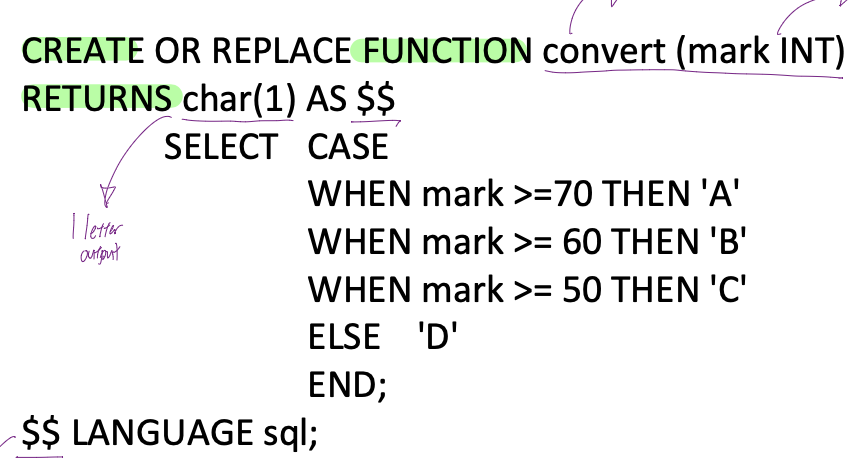
\includegraphics[width=0.55\linewidth]{13_func_atomic.png} \\
      \underline{Example Query:} \verb|SELECT Name, convert(Mark) FROM Scores;|
      \item \textbf{Returns 1 EXISTING tuple:}
      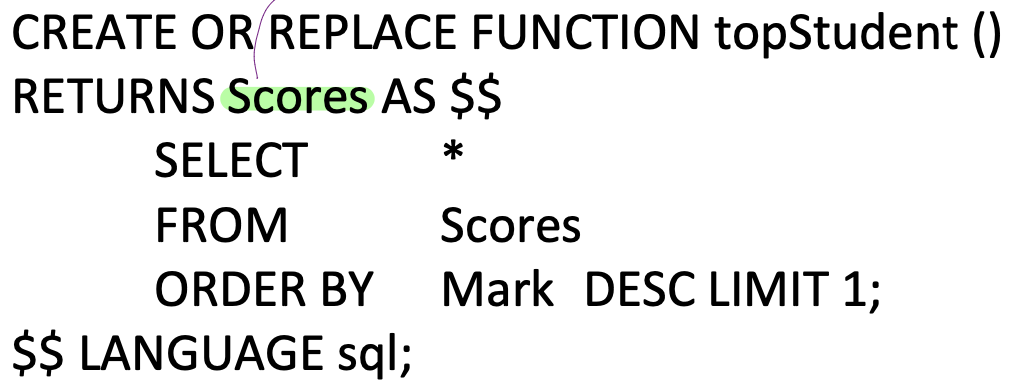
\includegraphics[width=0.55\linewidth]{14_func_existing.png} \\
      \underline{Example Query:} \verb|SELECT topStudent();|
      \item \textbf{Returns EXISTING SET of tuples:}
      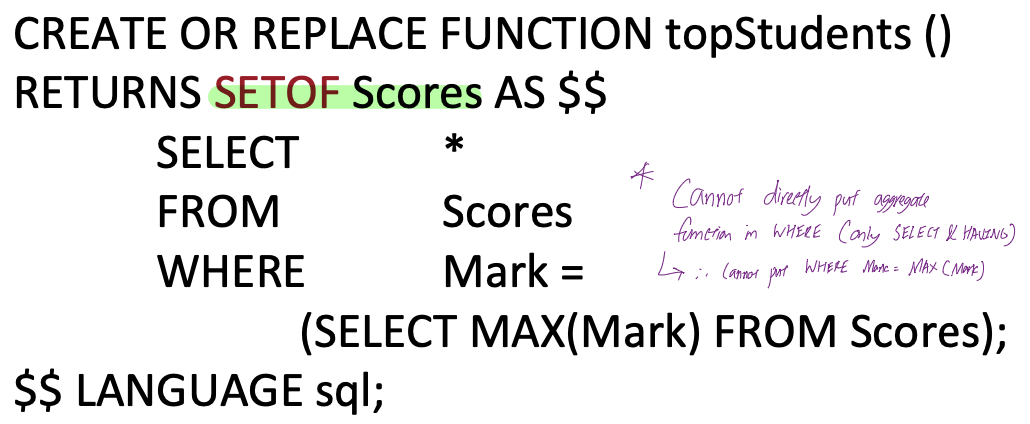
\includegraphics[width=0.55\linewidth]{15_func_existing_set.png} \\
      \underline{Example Query:} \verb|SELECT * FROM topStudents();|
      \item \textbf{Returns 1 NEW tuple (Note parameters):} \\
      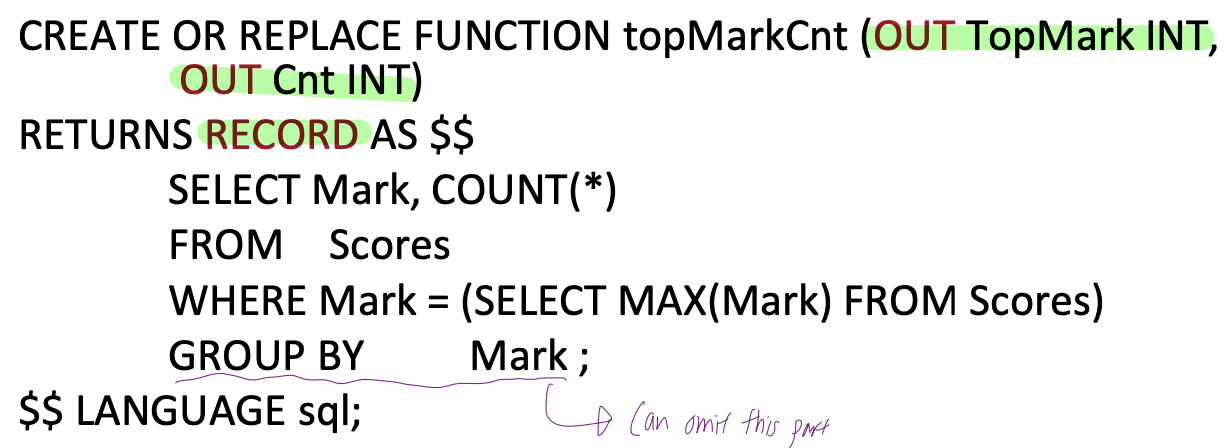
\includegraphics[width=0.65\linewidth]{16_func_new.png} \\
      \underline{Example Query:} \verb|SELECT topMarkCnt();|
      \item \textbf{Returns NEW SET of tuples (Note parameters):}
      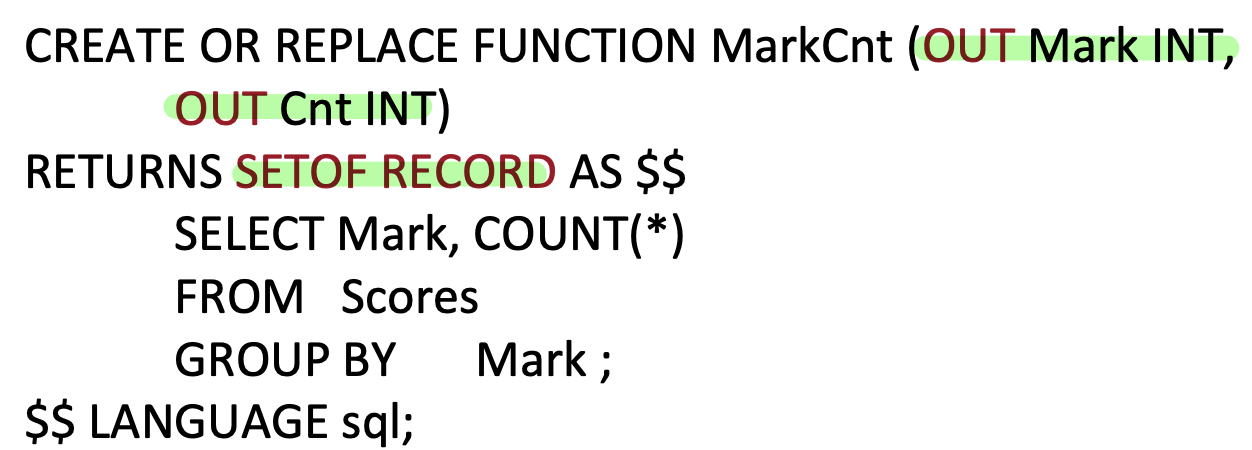
\includegraphics[width=0.55\linewidth]{17_func_new_set.png} \\
      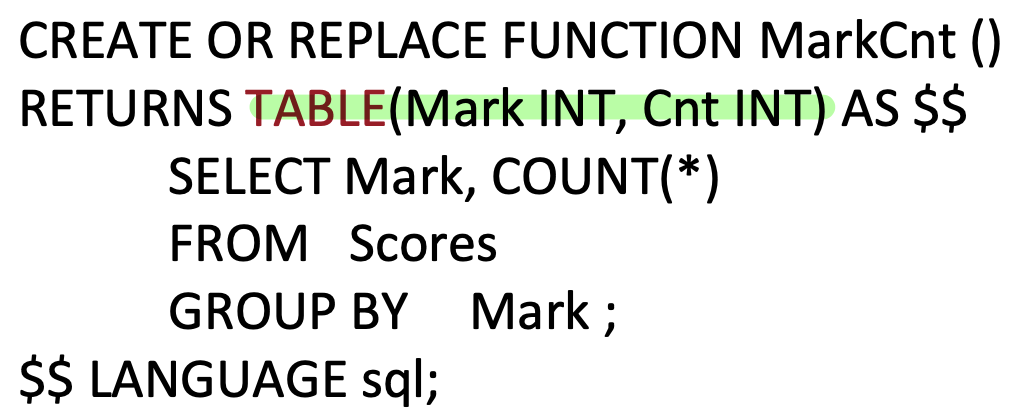
\includegraphics[width=0.55\linewidth]{18_func_new_table.png} \\
      \underline{Example Query:} \verb|SELECT MarkCnt();|
    \end{itemize}

    \subsection{Procedures}
    \begin{itemize}
      \item Do not return value/tuple, treated as a transaction
      \item \underline{Syntax}: \verb|CREATE OR REPLACE PROCEDURE...|
    \end{itemize}
    \subsection{Control Structures:}
    \begin{enumerate}
      \item \verb|IF ... THEN ... ELSE ... END IF|
      \item \verb|LOOP ... END LOOP|
      \item \verb|EXIT ... WHEN ...|
      \item \verb|WHILE ... LOOP ... END LOOP|
      \item \verb|FOR ... IN ... LOOP ... END LOOP|
    \end{enumerate}

    \subsection{Variables:}
    \begin{itemize}
      \item Variables are declared in \verb|DECLARE| section, Actual function is in \verb|BEGIN ... END| section
      \item Values are selected into variables (\verb|SELECT COUNT(*) INTO| \verb|overlap_count|) OR assigned directly (\verb|temp_val := val1|)
    \end{itemize}

    \subsection{Cursor:}
    \begin{itemize}
      \item Cursor enables us to access each individual row selected by a \verb|SELECT| statement (DECLARE $\rightarrow$ OPEN $\rightarrow$ FETCH $\rightarrow$ CLOSE)
      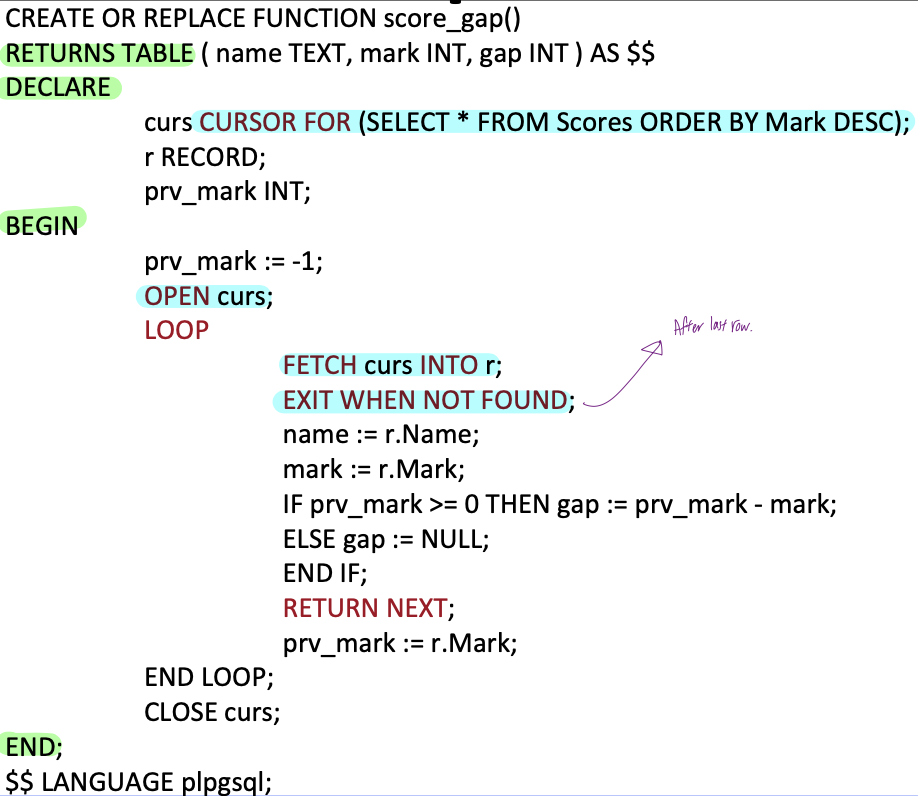
\includegraphics[width=0.7\linewidth]{19_cursor.png}
      \item \verb|OPEN|: SQL statement for cursor is executed \& cursor points to beginning of result
      \item \verb|FETCH|: Next tuple from cursor is read \& put into \verb|r| $\rightarrow$ No tuple, terminate loop
      \item \verb|RETURN NEXT|: Inserts a tuple to output of function
      \item \verb|CLOSE|: Releases resources allocated to cursor
      \item \underline{Cursor Movement:} \verb|FETCH PRIOR FROM cur INTO r|, \verb|FETCH| \verb|FIRST FROM cur INTO r|, \verb|FETCH LAST FROM cur INTO r|, \verb|FETCH ABSOLUTE x FROM cur INTO r| (fetch x\textsuperscript{th} tuple)
    \end{itemize}

    \section{Triggers}
    \subsection{Basics of Triggers \& Trigger Functions}
    \textbf{Triggers:} Condition that database has to check whenever appropriate \\
    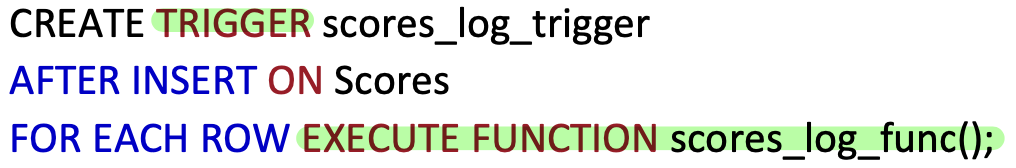
\includegraphics[width=0.7\linewidth]{20_trigger.png} \\
    \begin{itemize}
      \item Tells database to watch out for insertions on Scores $\rightarrow$ Calls \verb|scores_log_func()| after each insertion of a tuple
    \end{itemize}
    \textbf{Trigger Functions:} Expression of the condition about something done to database
    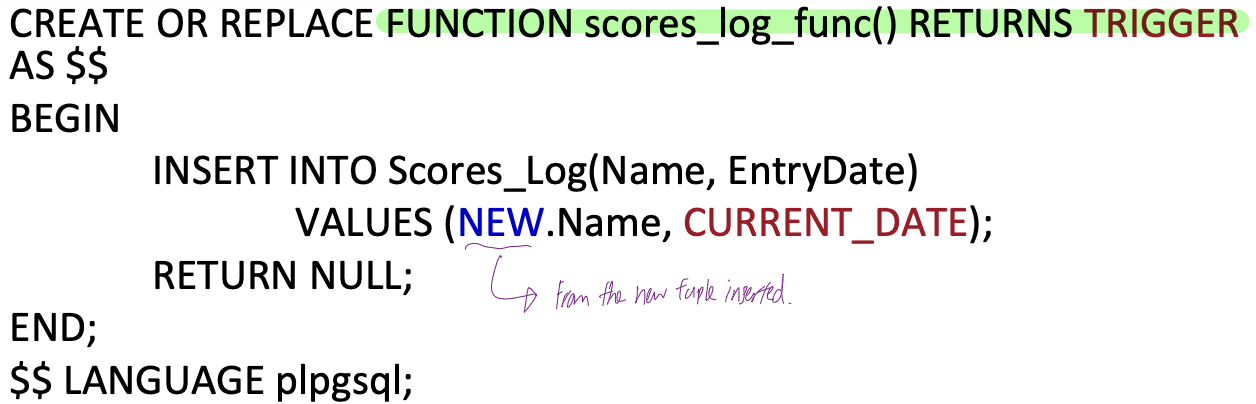
\includegraphics[width=0.8\linewidth]{21_trigger_func.png}
    \begin{itemize}
      \item \verb|RETURNS TRIGGER| indicates that this is a trigger function (Only TRIGGER functions have access to \verb|NEW| keyword)
      \item Trigger functions should not have any input parameters
      \item Trigger functions can access
      \begin{enumerate}
        \item \verb|TG_OP|: Operation that activated trigger (INSERT, UPDATE, DELETE)
        \item \verb|TG_TABLE_NAME|: Name of table that activated trigger
        \item \verb|OLD|: Old tuple being updated/deleted
        \item \verb|NEW|: New tuple to update/ to be inserted
      \end{enumerate}
    \end{itemize}

    \subsection{Trigger Operations}
    \begin{enumerate}
      \item \textbf{Insert:} OLD (NULL tuple) $\vert$ NEW (Non-NULL tuple)
      \item \textbf{Update:} OLD (Non-NULL tuple) $\vert$ NEW (Non-NULL tuple)
      \item \textbf{Delete:} OLD (Non-NULL tuple) $\vert$ NEW (NULL tuple)
    \end{enumerate}

    \subsection{Trigger Timing}
    \begin{enumerate}
      \item \textbf{AFTER:} Function would be executed AFTER tuple operation
      \begin{itemize}
        \item \underline{AFTER INSERT:} Return value does not matter
        \item \underline{AFTER UPDATE:} Return value does not matter
        \item \underline{AFTER DELETE:} Return value does not matter
        \item Reason: Trigger function is invoked after main operation is done
      \end{itemize}
      \item \textbf{BEFORE:} Function would be executed BEFORE tuple operation
      \begin{itemize}
        \item \underline{BEFORE INSERT:} Non-NULL tuple returned $\rightarrow$ tuple will be inserted $\vert$ NULL tuple returned $\rightarrow$ no tuple inserted
        \item \underline{BEFORE UPDATE:} Non-NULL tuple returned $\rightarrow$ tuple will be updated tuple $\vert$ NULL tuple returned $\rightarrow$ no tuple updated
        \item \underline{BEFORE DELETE:} Non-NULL tuple returned $\rightarrow$ deletion proceeds as normal $\vert$ NULL tuple returned $\rightarrow$ no deletion
        \item \verb|RETURN NULL|: Tells database to ignore rest of operation
      \end{itemize}
      \item \textbf{INSTEAD OF:} Function would be executed INSTEAD OF tuple operation (Can be defined on views only, instead of doing something on a view, do it on a table)
      \begin{itemize}
        \item \underline{Returning NULL}: Signals database to ignore rest of operation on current row
        \item \underline{Returning non-NULL tuple}: Signals database to proceed as normal
      \end{itemize}
    \end{enumerate}

    \subsection{Trigger Levels}
    \begin{itemize}
      \item \textbf{FOR EACH ROW}: Row-level trigger that executes trigger function for every tuple encountered
      \item \textbf{FOR EACH STATEMENT}: Statement-level trigger that executes trigger function only once
      \begin{itemize}
        \item Statement-level triggers ignore values returned by trigger operations, \verb|RETURN NULL| will not make database omit subsequent operations $\rightarrow$ Need to RAISE EXCEPTION instead of RAISE NOTICE to prevent deletion
      \end{itemize}
      \item \verb|INSTEAD OF| only allowed on row-level
      \item \verb|BEFORE/AFTER| allowed on both row-level \& statement-level
    \end{itemize}

    \subsection{Trigger Condition}
    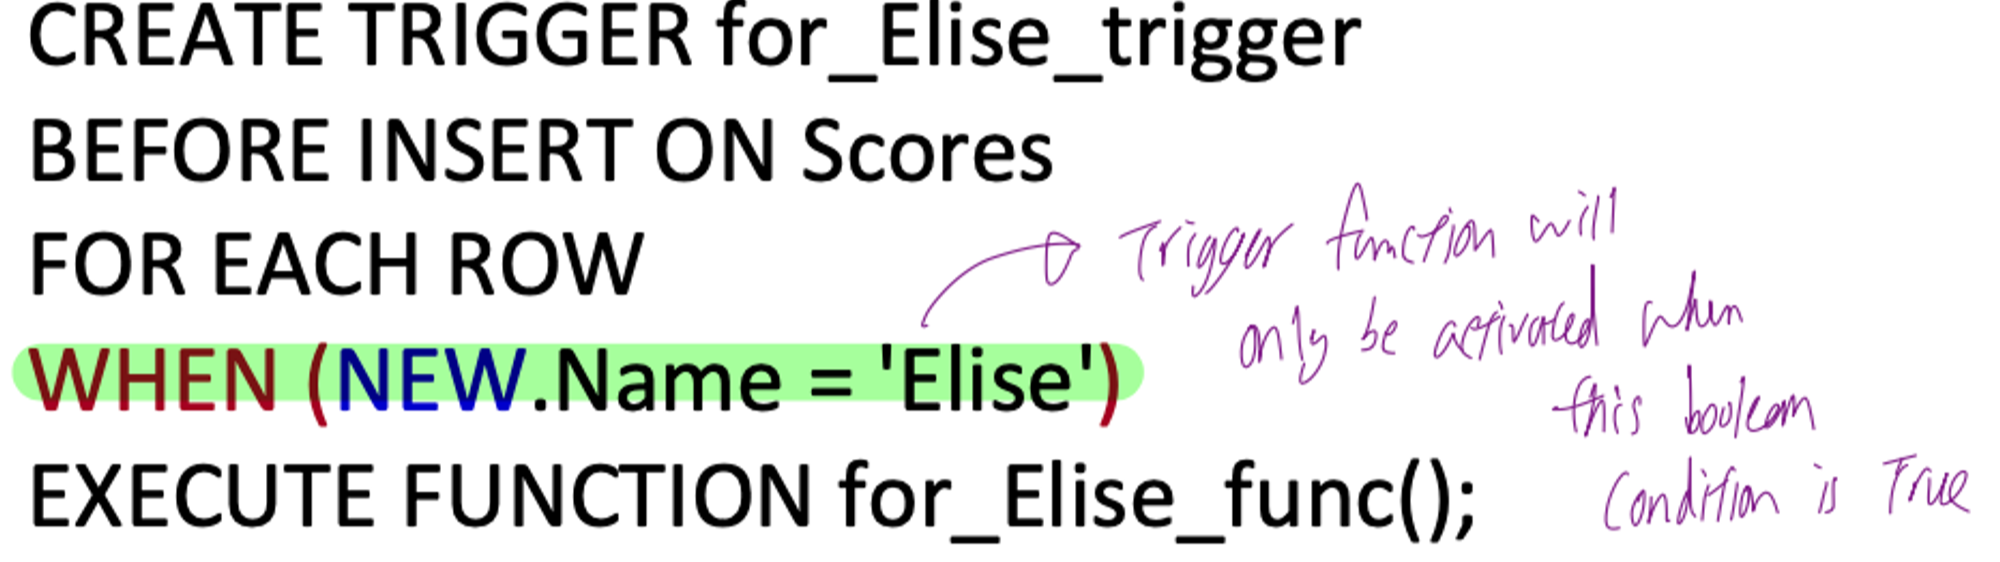
\includegraphics[width=0.7\linewidth]{22_trigger_condition.png}
    \begin{itemize}
      \item No \verb|SELECT| in \verb|WHEN()|
      \item No OLD in \verb|WHEN()| for \verb|INSERT|
      \item No NEW in \verb|WHEN()| for \verb|DELETE|
      \item No \verb|WHEN()| for INSTEAD OF
    \end{itemize}

    \subsection{Deferred Trigger}
    \begin{itemize}
      \item Defers checking of triggers
      \item \textbf{Syntax:}
      \begin{itemize}
        \item \verb|CONSTRAINT| and \verb|DEFERRABLE| together $\rightarrow$ Trigger can be deferred
        \item \verb|INITIALLY DEFERRED| by default $\rightarrow$ Trigger is deferred
        \item \verb|INITIALLY IMMEDIATE| $\rightarrow$ Trigger is not deferred by default
        \item Deferred triggers only works with AFTER (to defer trigger, has to execute after main operation) \& FOR EACH ROW
      \end{itemize}
      \item \textbf{Procedure:}
      \begin{enumerate}
        \item Put inter-dependent statements into 1 transaction
        \item Defer trigger check to end of transaction (Trigger is activated at COMMIT)
      \end{enumerate}
      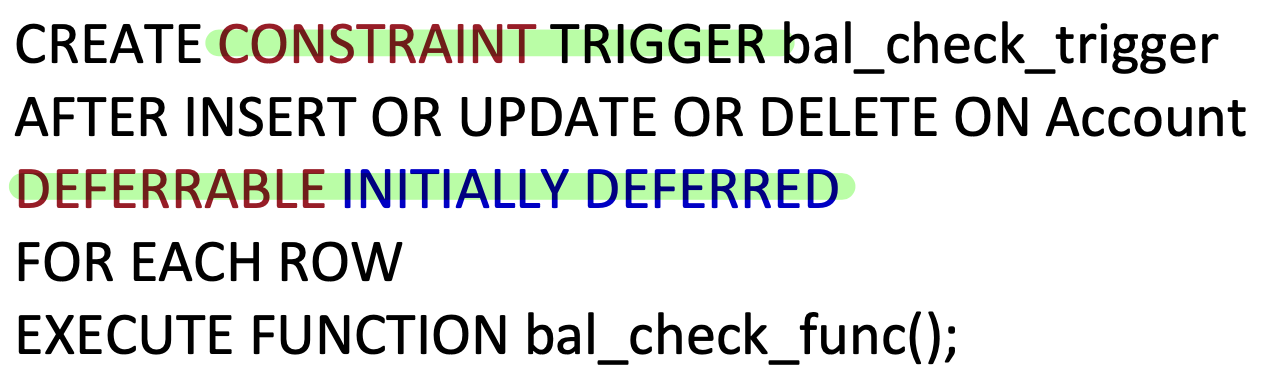
\includegraphics[width=0.6\linewidth]{23_trigger_defer_1.png}
      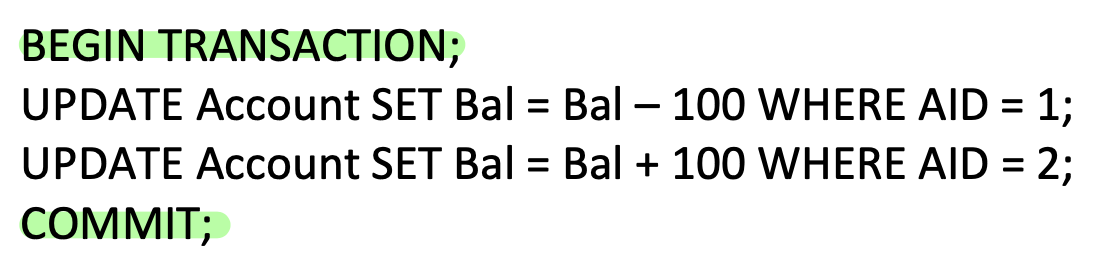
\includegraphics[width=0.6\linewidth]{24_trigger_defer_2.png}
      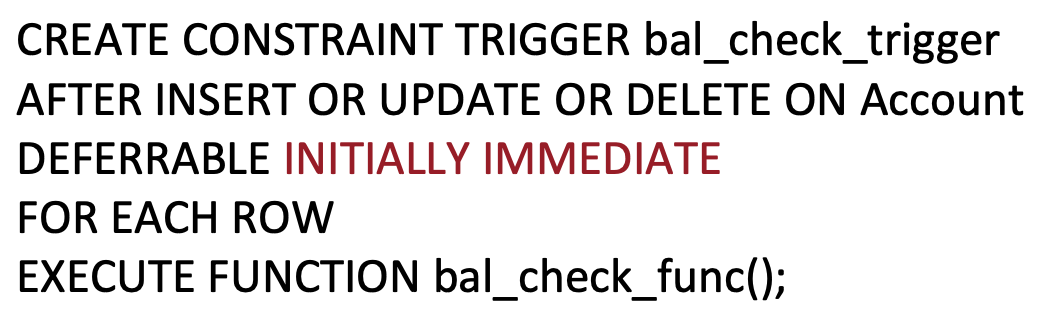
\includegraphics[width=0.6\linewidth]{25_trigger_defer_3.png}
      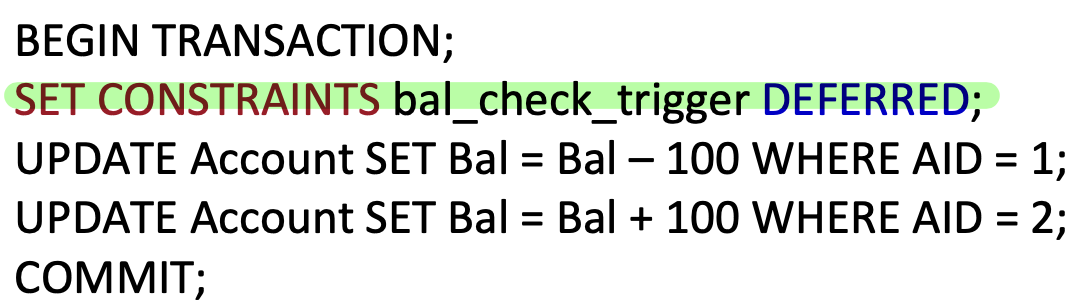
\includegraphics[width=0.6\linewidth]{26_trigger_defer_4.png}
    \end{itemize}

    \subsection{Multiple Triggers}
    \begin{itemize}
      \item \textbf{Order of trigger activation:}
      \begin{enumerate}
        \item BEFORE statement-level triggers
        \item BEFORE row-level triggers
        \item AFTER row-level triggers
        \item AFTER statement-level triggers
      \end{enumerate}
      \item Within each category, triggers are activated in alphabetical order
      \item If BEFORE row-level trigger returns NULL $\rightarrow$ subsequent triggers on same row are omitted
    \end{itemize}

    \section{Functional Dependencies}
    \subsection{Functional Dependency}
    \begin{itemize}
      \item \textbf{Definition:} If attribute $A$ uniquely decides attribute $B \rightarrow$ there is a FD from $A$ to $B$ ($A \rightarrow B$)
      \item \textbf{Formal Definition:} $A_1A_2...A_n \rightarrow B_1B_2...B_n$ if whenever 2 objects have the same values on $A_1A_2...A_n$, they always have same values on $B_1B_2...B_n$
      \item \textbf{FDs on Tables:} An FD may hold on 1 table but does not hold on another
      \item \textbf{Techniques to spot FDs:}
      \begin{enumerate}
        \item Given $A \rightarrow B$ \& A is FALSE, the FD is vacuously TRUE (A is FALSE means that there are no $\geq$ 2 tuples having same $A$ values)
        \item Come up with a counter example to the requirement \& put column with same values on the LHS, column with different values on the RHS (Eg. No 2 customers buy the same product: $C_1,P_1$ \& $C_2,P_1$ violates requirement $\rightarrow$ Place P on LHS, place C on RHS ($P \rightarrow C$))
      \end{enumerate}
    \end{itemize}
    \subsection{Armstrong Axioms \& Rules}
    \begin{enumerate}
      \item \textbf{Reflexivity:} $AB \rightarrow A$
      \item \textbf{Augmentation:} If $A \rightarrow B$ then $AC \rightarrow BC$
      \item \textbf{Transitivity:} If $A \rightarrow B$ and $B \rightarrow C$ then $A \rightarrow C$
      \item \textbf{Decomposition:} If $A \rightarrow BC$ then $A \rightarrow B$ and $A \rightarrow C$
      \item \textbf{Union:} If $A \rightarrow B$ and $A \rightarrow C$ then $A \rightarrow BC$
    \end{enumerate}
    \subsection{Closure}
    \begin{itemize}
      \item \textbf{Definition:} $\{A_1,A_2,...,A_n\}^{+}$ = Set of attributes that can be decided by $A_1,A_2,...,A_n$ directly or indirectly
      \item \textbf{Computing Closures:}
      \begin{enumerate}
        \item Initialise closure to $\{A_1,A_2,...,A_n\}$
        \item If there is an FD: $A_i,A_j,...,A_m \rightarrow B$, such that $A_i,A_j,...,A_m$ are all in closure, then put B into closure
        \item Repeat step 2 until we cannot find any new attribute to put into closure
      \end{enumerate}
      \item \textbf{Using Closures to prove FDs:}
      \begin{itemize}
        \item To prove that $A \rightarrow B$ holds, only need to show that $\{A\}^{+}$ contains B
        \item To prove that $A \rightarrow B$ does not hold, only need to show that $\{A\}^{+}$ does not contain B
      \end{itemize}
    \end{itemize}

    \subsection{Keys, Superkeys, Prime Attributes}
    \begin{itemize}
      \item \textbf{Superkeys of a table:} Set of attributes in a table that decides all other attributes
      \item \textbf{Keys of a table:} A superkey that is minimal (If we remove any attribute from superkey, it will not be a superkey anymore $\vert$ A table may have multiple keys)
      \item \textbf{Prime Attribute:} If an attribute appears in a key, then it is a prime attribute
    \end{itemize}
    \textbf{Algorithm for finding keys}: Given table $T(A,B,C...)$ and a set of FDs on $T$
    \begin{enumerate}
      \item Consider every subset of attributes in$T$
      \item Derive the closure of each subset
      \item Identify all superkeys based on closures (Pick closures that contain all attributes of $T$)
      \item Identify all keys from superkeys
      \\ \underline{Tricks:} (1): Check all small attribute sets first (If closure of the set contains all attributes, no need to check superset already) $\vert$ (2): If an attribute does not appear on RHS of any FD, then it must be in every key
    \end{enumerate}

    \section{BCNF}
    \subsection{Non-trivial \& Decomposed FD}
    \begin{itemize}
      \item \textbf{Decomposed FD:} An FD whose RHS has only 1 attribute (A non-decomposed FD can always be transformed into a set of decomposed FDs via Rule of Decomposition)
      \item \textbf{Types of FDs:}
      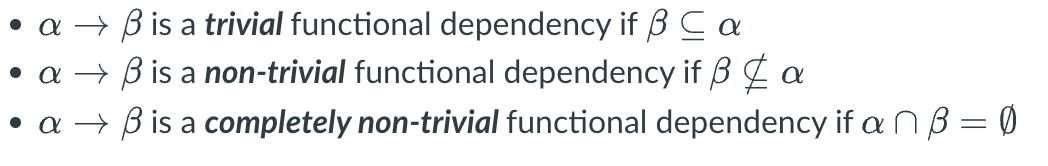
\includegraphics[width=0.9\linewidth]{27_fd.png}
      \item \textbf{Non-trivial \& Decomposed FD} A decomposed FD whose RHS does not appear in LHS
      \item \textbf{Algorithm for finding Non-trivial \& decomposed FDs (via Closures)}: Consider $R(A,B,C)$
      \begin{enumerate}
        \item Consider all attribute subsets in $R$
        \item Compute closure of each subset
        \item From each closure, remove trivial attributes (remove attributes from closure that appear in original subset)
        \item Derive non-trivial \& decomposed FDs from each closure (use Rule of Decomposition if needed)
      \end{enumerate}
    \end{itemize}

    \subsection{BCNF}
    \begin{itemize}
      \item \textbf{Definition:} Table $R$ is in BCNF if every non-trivial \& decomposed FD has a superkey in its LHS
      \item \textbf{Algorithm to check BCNF:}
      \begin{enumerate}
        \item Compute closure of each attribute subset
        \item Derive keys of $R$ (using closure)
        \item Derive all non-trivial \& decomposed FDs on $R$ (using closure)
        \item Check if all non-trivial \& decomposed FDs' LHS is a superkey $\rightarrow$ if all non-trivial \& decomposed FDs satisfy requirement, R is in BCNF
      \end{enumerate}
      \item \textbf{Simplified Algorithm to check BCNF:}
      \begin{enumerate}
        \item Compute closure of each attribute subset
        \item Check if there is a closure such that it satisfies "more than but not all" condition
        \item If such a closure exists $\rightarrow$ R is NOT in BCNF
      \end{enumerate}
      \item \textbf{Properties of BCNF:}
      \begin{enumerate}
        \item No update or deletion or insertion anomalies
        \item Small redundancy
        \item Original table can always be reconstructed from decomposed tables
        \item Dependencies may not be preserved in decomposed table
      \end{enumerate}
    \end{itemize}

    \subsection{BCNF Decomposition}
    If table is not in BCNF $\rightarrow$ Decompose table into smaller tables (Normalisation)
    \begin{itemize}
      \item \textbf{Decomposition Algorithm:}
      \begin{enumerate}
        \item Find a subset $X$ of attributes in $R$ such that its closure satisfies "more but not all" condition
        \item Decompose $R$ into 2 tables $R_1, R_2$ such that $R_1$ contains all attributes in $\{X\}^{+}$ \& $R_2$ contains all attributes in $X$ as well as attributes not in $\{X\}^{+}$
        \item If $R_1$ is not in BCNF $\rightarrow$ decompose $R_1$, If $R_2$ is not in BCNF $\rightarrow$ decompose $R_2$ 
      \end{enumerate}
    NOTE: BCNF decomposition of a table may not be unique $\vert$ Table only has 2 attributes $\rightarrow$ Table MUST be in BCNF
    \item \textbf{Projection of Closures/FDs:} Used when we want to derive closures on a table $R_i$ that is decomposed from a table $R \rightarrow$ Can decide whether $R_i$ is in BCNF \& whether to decompose $R_i$
    \begin{enumerate}
      \item Enumerate attribute subsets of $R_i$
      \item For each subset, derive its closure on $R$ (basically use FDs from $R$)
      \item Project each closure onto $R_i$ by removing those attributes that do not appear in $R_i$
    \end{enumerate}
    \item \textbf{Lossless Join Decomposition}
    \begin{itemize}
      \item Decomposition guarantees lossless join whenever common attributes in $R_1$ \& $R_2$ is a superkey of  $R_1$ or $R_2$
      \item \underline{WORKING}: For LJD with multiple decomposed schema, working only requires 1 possible decomposition \& show the working that each step is a LJD $\vert$ For non-LJD, working requires exploration of all possibilities \& explain why each possibility is non-LJD 
      \item BCNF guarantees lossless join
    \end{itemize}
    \end{itemize}

    \section{3NF}
    \subsection{Dependency Preservation}
    \begin{itemize}
      \item Let $S$ be given set of FDs on original table, $S'$ be set of FDs on decomposed table
      \item Decomposition preserves all FDs $\leftrightarrow$ $S$ \& $S'$ are equivalent (Every FD in $S'$ can be derived from $S$, Every FD in $S$ can be derived from $S'$)
    \end{itemize}

    \subsection{3rd Normal Form}
    \begin{itemize}
      \item \textbf{Definition:} A table satisfies 3NF $\leftrightarrow$ For every non-trivial \& decomposed FD either (1) LHS is a superkey or (2) RHS is a prime attribute (appears in a key)
      \item \textbf{Properties of 3NF:}
      \begin{enumerate}
        \item Not as strict as BCNF
        \item Small redundancy (not as small as BCNF)
        \item Lossless join property
        \item Preserves all FDs
      \end{enumerate}
      \item \textbf{BCNF VS 3NF:} Satisfying BCNF $\rightarrow$ Satisfying 3NF (but not necessarily vice versa) $\vert$ Violating 3NF $\rightarrow$ Violating BCNF (but not necessarily vice versa)
      \item \textbf{Algorithm to check 3NF:}
      \begin{enumerate}
        \item Derive keys of $R$ (via Algorithm to find keys)
        \item For each given FD, check if LHS is a superkey OR Each attribute on RHS is a prime attribute
        \item If all given FDs satisfy this condition $\rightarrow$ R is in 3NF
      \end{enumerate}
    \end{itemize}

    \subsection{3NF Decomposition}
    A table is NOT in 3NF $\rightarrow$ Decompose it into smaller tables that are in 3NF
    \begin{itemize}
      \item \textbf{BCNF Decomposition VS 3NF Decomposition:} BCNF Decomposition may perform $\geq$ 1 binary splits, each of which divides a table into 2 $\vert$ 3NF decomposition has only 1 split, which divides table into $\geq$ 2 parts
      \item \textbf{3NF Decomposition Algorithm:}
      \begin{enumerate}
        \item Given a table $R$ and a set $S$ of FDs, derive \underline{minimal basis} of S
        \item In minimal basis, combine FDs whose LHSs are the same (Basically get non-decomposed FDs aka. Canonical minimal basis)
        \item Create a table for each FD remained
        \item If none of the tables contains a key of original table $R$, create a table that contains any key of $R$ (Ensure lossless join decomposition)
        \item Remove subsumed tables (Remove table if all of its attributes are contained in another table)
      \end{enumerate}
    \end{itemize}

    \subsection{Minimal Basis}
    \begin{itemize}
      \item Minimal Basis of $S$ is a simplified version of S
      \item \textbf{Conditions:}
      \begin{enumerate}
        \item Every FD in minimal basis can be derived from $S$, and vice versa
        \item Every FD in minimal basis is a non-trivial \& decomposed FD
        \item No FD in minimal basis is redundant (No FD in minimal basis can be derived from other Fds in minimal basis)
        \item For each FD in minimal basis, none of attributes on LHS is redundant (If we remove an attribute from LHS, then resulting FD is a new FD that cannot be derived from original set of FDs)
      \end{enumerate}
      \item \textbf{Algorithm to find Minimal Basis}
      \begin{enumerate}
        \item Transform FDs, so that each RHS contains only 1 attribute (Decompose FDs)
        \item Remove redundant attributes on LHS of each FD
        \begin{enumerate}[label=\alph*]
          \item Given $AB \rightarrow C$, remove $A$ to produce $B \rightarrow C$
          \item Check whether $B \rightarrow C$ is implied by $S$ (Check if closure of $B$ contains $C$)
          \item If $B \rightarrow C$ is not implied, $A$ is NOT redundant, If $B \rightarrow C$ is implied, $A$ is redundant
        \end{enumerate}
        \item Remove redundant FDs (Remove FD from $S$ \& see if that FD can be derived from other FDs in $S$)
      \end{enumerate}
    \end{itemize}

    \subsection{Primary Keys \& FDs}
    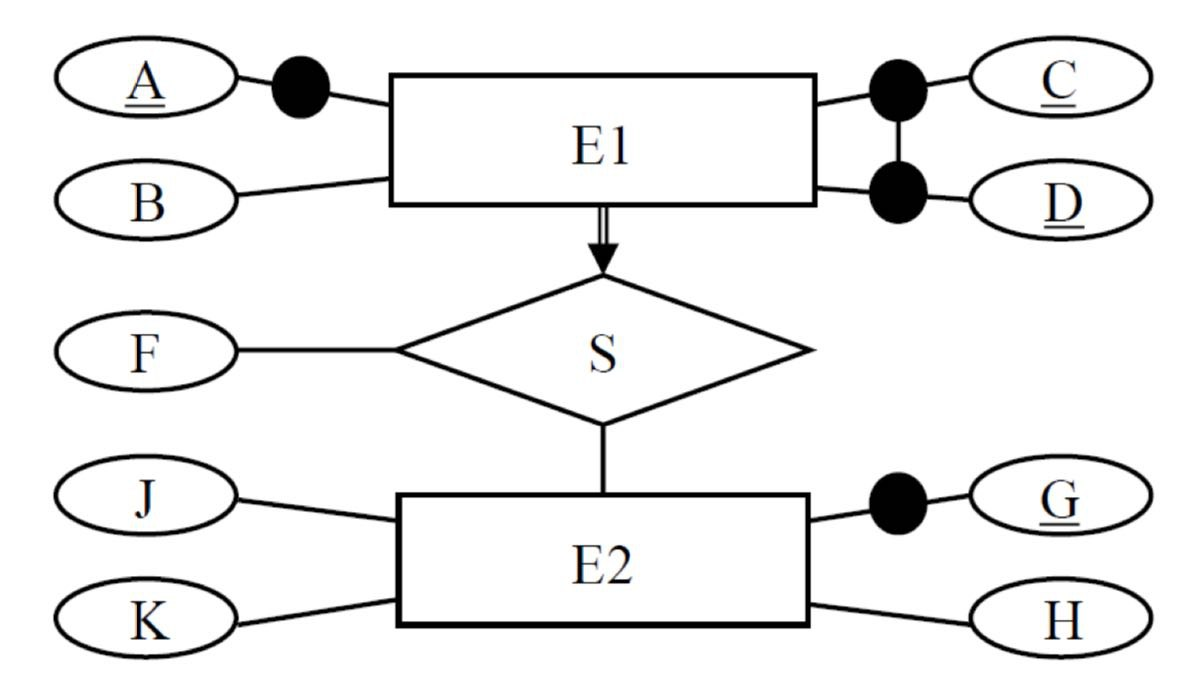
\includegraphics[width=0.8\linewidth]{28_fd_diagram.jpg}
    \begin{itemize}
      \item \textbf{Candidate Keys:} A, CD for E1 $\vert$ G for E2
      \item \textbf{Functional Dependencies:} A $\rightarrow$ CD, CD $\rightarrow$ A, A $\rightarrow$ B, CD $\rightarrow$ B, A $\rightarrow$ F, CD $\rightarrow$ F, A $\rightarrow$ G, CD $\rightarrow$ G, G $\rightarrow$ HJK 
    \end{itemize}
  \end{multicols*}
\end{document}
